\begin{table}[h]
    \centering
    \caption{Comparação do Tempo entre os algoritmos com entrada crescente.}
    \begin{tabular}{|c|c|c|c|c|c|c|}
        \hline
        Tamanho de Entrada & 10 & 100 & 1000 & 10000 & 100000 & 1000000 \\
        \hline
        Insertion Sort & 0.000000 & 0.000000 & 0.000000 & 0.000000 & 0.000000 & 0.003000 \\
        \hline
        Selection Sort & 0.000000 & 0.000000 & 0.001000 & 0.103000 & 10.177000 & 1089.101000 \\
        \hline
        Shell Sort & 0.000000 & 0.000000 & 0.000000 & 0.000000 & 0.004000 & 0.063000 \\
        \hline
        Bubble Sort & 0.000000 & 0.000000 & 0.001000 & 0.098000 & 9.734000 & 952.523000 \\
        \hline
    \end{tabular}
    \label{tab:comparacaogeral}
\end{table}

Observando à Tabela \ref{tab:comparacaogeral} e o gráfico \ref{fig:geral1} percebemos que quando se trata da entrada no melhor caso, ou seja, com números já ordenados, os algoritmos Insertion Sort e Shell sort continuam tendo uma boa performance até mesmo com valores muito altos de entrada, permanecendo com o tempo de ordenação próximo ao zero, já o Selection Sort e o Bubble sorte, mantém um bom tempo de execução com valores baixo mas quando se trata de muitas entradas eles gastam muito tempo para percorrer todo o vetor, pois mesmo já estando alternados os números eles precisam conferir todos até o final, não sendo uma boa escolha.

\begin{figure}[h!]
    \centering
    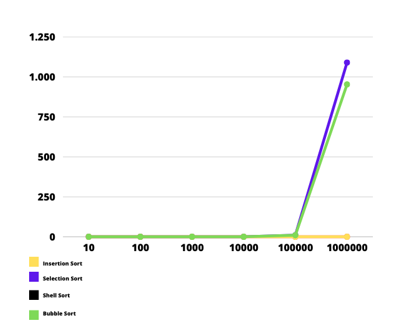
\includegraphics[width = 10cm]{Imagens/Geral/geral2.png}
    \caption{Gráfico de tempo entre os algoritmos com entrada crescente.}
    \label{fig:geral1}
\end{figure}
\newpage

\begin{table}[h]
    \centering
    \caption{Comparação do Tempo entre os algoritmos com entrada decrescente.}
    \begin{tabular}{|c|c|c|c|c|c|c|}
        \hline
        Tamanho de Entrada & 10 & 100 & 1000 & 10000 & 100000 & 1000000 \\
        \hline
        Insertion Sort & 0.000000 & 0.000000 & 0.001000 & 0.111000 & 10.856000 & 1088.031000 \\
        \hline
        Selection Sort & 0.000000 & 0.000000 & 0.000000 & 0.098000 & 9.769000 & 1046.444000 \\
        \hline
        Shell Sort & 0.000000 & 0.000000 & 0.000000 & 0.001000 & 0.007000 & 0.083000 \\
        \hline
        Bubble Sort & 0.000000 & 0.000000 & 0.002000 & 0.172000 & 17.373000 & 1697.082000 \\
        \hline
    \end{tabular}
    \label{tab:comparacaogeral2}
\end{table}

Enquanto para o pior caso, na Tabela \ref{tab:comparacaogeral2}, o único algoritmo que apresente uma diferença relevante com o melhor caso, é o Insertion Sort, que precisa percorrer e inverter todo o vetor para ordenar todos os números, tornando-o assim uma escolha inviável para entradas descrescentes quando se trata de um grande número de entradas no algoritmo.

\begin{figure}[h!]
    \centering
    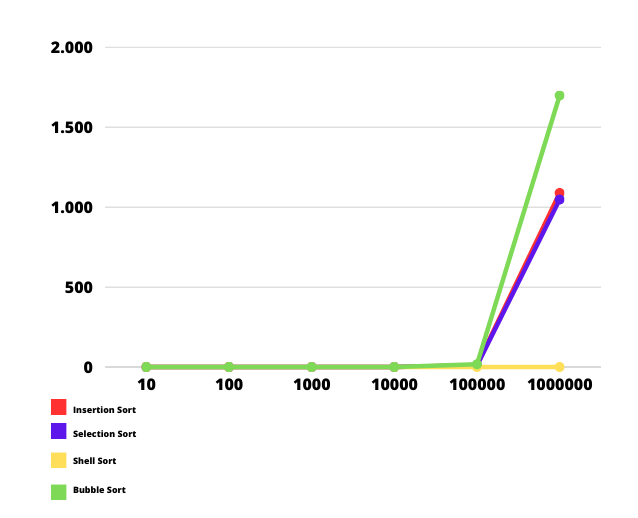
\includegraphics[width = 10cm]{Imagens/Geral/Captura de tela 2023-09-27 220558.png}
    \caption{Gráfico de tempo entre os algoritmos com entrada decrescente.}
    \label{fig:geral2}
\end{figure}
\newpage
